\question {
    假设一个程序有两个段,其中段 0 保存代码指令,段 1 保存读写的数据。段 0 的权限是可读可执行,
    段 1 的权限是可读可写,如下所示。该程序运行的内存系统提供的虚址空间为 14-bit 空间,其中
    低 10-bit 为页内偏移,高 4-bit 为页号。
}

\begin{figure}[H]
    \centering
    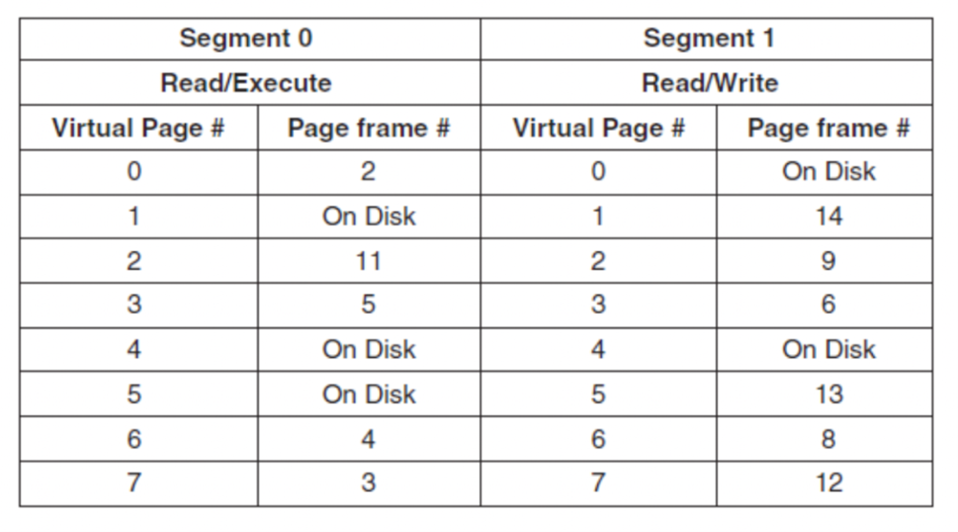
\includegraphics[width=0.6\textwidth]{img/9_3.png}
\end{figure}

当有如下的访存操作时,请给出每个操作的实际访存物理地址或是产生的异常类型(例如缺页异常、权限异常等)

\begin{parts}
    \part 读取段 1 中 page 1 的 offset 为 3 的地址
    \part 向段 0 中 page 0 的 offset 为 16 的地址写入
    \part 读取段 1 中 page 4 的 offset 为 28 的地址
    \part 跳转至段 1 中 page 3 的 offset 为 32 的地址
\end{parts}

\begin{solution}

% Table generated by Excel2LaTeX from sheet 'Sheet1'
\begin{tabular}{|c|c|c|c|c|c|}
    \hline
    seg   & vpn   & offset & ppn   & pa    & excp \bigstrut\\
    \hline
    1     & 1     & 3     & 14    & 0x3803 & 无异常 \bigstrut\\
    \hline
    0     & 0     & 16    & 2     & 0x810 & 权限异常 \bigstrut\\
    \hline
    1     & 4     & 28    & 无     & 无     & 缺页异常 \bigstrut\\
    \hline
    1     & 3     & 32    & 6     & 0x1820 & 权限异常 \bigstrut\\
    \hline
\end{tabular}%


\end{solution}